%!TEX root = ./main.tex

\documentclass[aspectratio=169,t,xcolor=table]{beamer}
\usepackage[utf8]{inputenc}
\usepackage{booktabs} 
\usepackage{subcaption}
\usepackage{src/stylings/main}

\usepackage[utf8]{inputenc}
\usepackage[T1]{fontenc}
\usepackage{hyperref}
\usepackage{csquotes}
\usepackage[
	backend=biber,
	style=numeric,
	citestyle=numeric,
	sorting=none,
	url=false]{biblatex}

\setbeamertemplate{bibliography item}[text]
\renewcommand*{\bibfont}{\scriptsize}
\addbibresource{src/bib/cites.bib}
\addbibresource{src/bib/web.bib}

\usepackage{array}
\usepackage{tabularx}
\usepackage{lipsum}
\setcounter{tocdepth}{3}

\usepackage{appendixnumberbeamer}
\usepackage{listings}
\usepackage{graphicx}
\graphicspath{{assets/}}

\title{Mapping GraphQL to the Haskell Type System}
\subtitle{Bachelor Thesis}
\institute[UHH] 
{
  University of Hamburg \\ 
  Faculty of Mathematics, Informatics and Natural Sciences (MIN) \\
  B.Sc. Human‐Computer Interaction (HCI)

}
\date{08.02.2020}
\author{Daviti Nalchevanidze}

\begin{document}
\setLogos{assets/logo/uhh.pdf}{assets/logo/uhh-compact.pdf} 
\setLayout{titlepage}
\frame[noframenumbering]{\titlepage}
\setLayout{regular} 
%!TEX root = ../../main.tex

\frame[noframenumbering]{\titlepage}

\begin{frame}
    \frametitle{Table of Contents}
    \tableofcontents
\end{frame}
\newcommand{\importGQL}[2]{
    \lstinputlisting[
        caption={#2},
    ]{src/code/#1.gql}   
}

\newcommand{\importHS}[2]{
    \lstinputlisting[
        language={haskell},
        caption={#2},
    ]{src/code/#1.hs}   
}

\newcommand{\importHSFragment}[4]{
    \lstinputlisting[
        language={haskell},
        caption={#4},
        firstline=#2, 
        lastline=#3,
    ]{src/code/#1.hs}   
}

\newcommand{\expr}[1]{\hspace{0.2mm}\mbox{\textcolor{green!35!blue!55!black}{\texttt{#1}}}}

\newcommand{\li}[1]{\item \textcolor{black}{\textbf{#1}}:}

\section{Introduction}

\begin{frame}\frametitle{Introduction}

    \begin{block}{Current Challenges}
        Modern web applications continuously transfer large amounts of data between clients and the server. They must be adaptable and available at any time, anywhere in the world, and support multiple devices. This presenting complexity, performance, and reliability challenges in development. 
    \end{block}

    \begin{block}{Haskell and  GraphQL}
        Haskell has proven to be safe and capable of managing the complexity. GraphQL enables clients to query only the data they need to improve performance, while servers can address multiple devices. Their combination can be useful to solve other problems.
    \end{block}

\end{frame}

\begin{frame}\frametitle{Motivation}

\begin{block}{GraphQL Haskell libraries}
    Existing GraphQL Haskell libraries either do not provide sufficient type safety or straightforward mapping, making them cumbersome to use.
\end{block}

\begin{block}{Objectives}
Our goal is to provide a library that requires minimal effort to use and provides a good developer experience while still guaranteeing reliability.
\end{block}

\end{frame}
%!TEX root = ../../main.tex
\section{Background}

\subsection{Haskell}
\begin{frame}\frametitle{Haskell}

Haskell is a non-strict, purely functional language with static typing and algebraic data types. Many developers think that Haskell programs look nice~\cite{history-of-haskell}.

\footnotesize

\begin{block}{Haskell is lazy}
    Laziness is a primary concern in Haskell's design. Technically, Haskell is a non-strict semantic language; lazy evaluation is merely an implementation technique for a non-strict language~\cite{history-of-haskell}.
\end{block}

\begin{block}{Haskell is pure}
Due to laziness, the evaluation sequence is demand-oriented, a function call can no longer guarantee reliable performance of side effects. Consequently, the pure design is inevitable~\cite{history-of-haskell}.
\end{block}

\end{frame}

\begin{frame}\frametitle{Algebraic Data Types}

Algebraic data types and pattern matching are fundamental to most modern functional languages~\cite{trees-that-grow}. Using pattern matching against algebraic data types improves readability significantly~\cite{history-of-haskell}.

An algebraic data type is the sum of one or more alternatives, where each alternative is a product of zero or more fields (Haskell also allows a sum of zero alternatives, the so-called empty type)~\cite{history-of-haskell}. 
        
\importHS{maybe}{Algebraic Data Types~\cite{history-of-haskell}}

Once a data type is defined and compiled, its definition cannot be extended by adding new data constructors or new fields~\cite{trees-that-grow}.

\end{frame}

\begin{frame}\frametitle{Records }

The record system provides syntactic sugar for what might otherwise be written using ordinary, positional, algebraic data type declarations~\cite{lw-ext-records}. 

\importHSFragment{records}{0}{4}{Haskell Record}

Haskell record are not extensible. There are no operators for adding and removing fields in a record, we cannot reuse labels between different record types~\cite{poly-ext-records, hlist,lw-ext-records}. 

\end{frame}

\begin{frame}\frametitle{Record Values}

Records bring significant advantages and greatly simplify programming with data structures that have many components. Since the individual components are accessed by name (not by position), the fields' ordering is not crucial~\cite{lw-ext-records}.

\importHSFragment{records}{6}{10}{Haskell Record Values}
% For example, 
% the data type Deity declares a regular algebraic data type, but at the same time, constructor field accessors and modifiers. 

\end{frame}

\begin{frame}\frametitle{Monads}

Pure languages facilitate changes by making the data visible on which each operation depends. However, a seemingly small change may require more extensive restructuring than impure functions.  Programming with monads solves this inflexibility and brings properties that are characteristic only of impure functions~\cite{essence-of-fp}.

monads are formed by a type constructor \expr{M} and a pair of functions,\expr{return} and \expr{>>=}~\cite{history-of-haskell,essence-of-fp}. The type \expr{M a} is a computation that returns a value of type \expr{a} and possibly performs some side effects~\cite{history-of-haskell}. The purpose of \expr{return} and \expr{>>=} is to push a value into computation and to evaluate a computation, yielding a value~\cite{essence-of-fp}.

Since the monad allows the compiler to determine impure and pure operations, the Haskell language can use specific optimizations. However, the developer still has the freedom to define their execution order~\cite{history-of-haskell}.

\end{frame}

\begin{frame}\frametitle{Datatype-Generic Programming}
    
Datatype-generic programming enables writing single functions that address various cases and types. The standard examples are parsing,  serialization, or comparing of data types~\cite{derivable-type-classes}. It increases the reliability of programs by reducing code duplication and improving reusability and modularity. it makes programming languages flexible while still guaranteeing safety~\cite{datatype-generic-programming,optimizing-generics}.
  
\importHS{generics}{Generic Deriving}. 
    
The basic idea behind it is to represent all types and values by a small set of data types, which are also called generic representation types. They are the building blocks of the structural representation of all other types~\cite{optimizing-generics}. the user can convert arbitrary types to their generic representation, operate on them, and convert them back to their original types~\cite{optimizing-generics,history-of-haskell, ghc-generics}.

\end{frame}
\subsection{GraphQL}

\begin{frame}\frametitle{GraphQL}

  \footnotesize
  \begin{block}{What is GraphQL?}
  GraphQL is an application layer framework for solving the efficiency problems of web communication~\cite{gql-iot}. It was developed internally at  Facebook for three years and published in 2016~\cite{initial-analysis-of-gql}. 
  \end{block}

  \begin{block}{GraphQL as current trend}
  Since its first appearance, it has gained a rich open-source ecosystem~\cite{gql-healthcare}, and the trust of companies from various sectors. e.g. (GitHub), entertainment (Netflix), finance (PayPal), travel (KLM), and others~\cite{morph-gql-1}.
  \end{block}

\begin{block}{Typed Query Language}
  GraphQL is a hierarchically structured language with a strongly typed schema~\cite{gql-healthcare}, where the type system (as a public schema) provides a solid contract between client and server and the possibility of errors caused by a part of the invalid request on the client~\cite{real-time-sys-arc-based-on-gql}.
\end{block}

\end{frame}

\begin{frame}\frametitle{Advantages and Disadvantages of GraphQL}

\footnotesize

\begin{block}{Over-Fetching and Under-Fetching}

reduces the number of JSON responses returned by API calls. which interesting for mobile applications, often faced with limited bandwidth and speed~\cite{migrating-to-gql,gql-healthcare}. In the studies showed that GraphQL could significantly improve performance by reducing unnecessary transfer costs and resulted in a significant reduction in energy consumption and transaction delays and even a reduction in response size~\cite{migrating-to-gql,real-time-sys-arc-based-on-gql,gql-iot}.
\end{block}

\begin{block}{API Versioning}

a stable and consistent contract between two systems for information exchange while remaining flexible for future changes~\cite{gql-healthcare}. 

\begin{itemize}
  \item new fields added to a type do not result in client changes~\cite{migrating-to-gql}. 
  \item provides an \expr{@deprecated} annotation for unsupported fields~\cite{migrating-to-gql}. 
\end{itemize}

\end{block}

\begin{block}{Facilitates Rapid Product Development}

GraphQL requires less effort to implement requirements than REST~\cite{rest-vs-gql-controlled-experiment}.

\begin{itemize}
  \item  GraphQL uses familiar syntax and semantics, similar to common programming languages, shortening the learning curve for beginners~\cite{rest-vs-gql-controlled-experiment}.
  \item GraphQL-IDEs enables real-time query validation and auto-completion~\cite{rest-vs-gql-controlled-experiment,migrating-to-gql}.
  \item Introspection frees up servers to support an interface description language and enables clients to explore the REST instantly~\cite{migrating-to-gql}. 
\end{itemize}

\end{block}

% Using GraphQL with Haskell has the following advantages: First, the languages are typed and support union types. Second, GraphQL fields are lazy, concurrent, resolvable functions that fit Haskell's non-strict and concurrent nature~\cite{gql-spec,haskell-homepage}. This way, the developer does not worry about laziness and concurrency and focuses on business logic.


\end{frame}

\begin{frame}\frametitle{Language}

\begin{block}{GraphQL Schema}

GraphQL allows the client to query a domain-specific database represented by a schema. The schema can be defined with a domain-specific language called Schema Definition Language (SDL)~\cite{migrating-to-gql,gql-on-graph-db}.


\end{block}

\begin{block}{GraphQL Queries}

GraphQL provides a query language that is used by clients. Every GraphQL query is defined in this language and sent to the single GraphQL endpoint as a simple string~\cite{migrating-to-gql,real-time-sys-arc-based-on-gql}.
The query is syntactically similar to JSON but follows the server's specific schema instead of arbitrary JSON objects~\cite{gql-on-graph-db,initial-analysis-of-gql}. 



To respond to queries, the developer of a GraphQL server must implement a function for each field of type resolver. These functions return query values from an underlying data structure.  The GraphQL engine calls them during the query and returns their value as a JSON document~\cite{migrating-to-gql,real-time-sys-arc-based-on-gql}. 


\end{block}


\end{frame}

\begin{frame}
\importGQL{schema}{Schema}
\end{frame}

\begin{frame}

\importGQL{query}{Sample GraphQL Query Using the Mythology }

\importJSON{response}{GraphQL Response of the Query}

\end{frame}


\section{Requirements}

\begin{frame}\frametitle{Requirements}  

\begin{alertblock}{Maintainability}

Maintainable software can adapt to the many changes occurring during software development.~\cite{requirements-change-1,view-of-web, sof-sus-institute-maintainability}

% It allows developers to quickly: fix bugs, add a new feature or increase performance without introducing new bugs

\begin{itemize}

    \li{Low boilerplate} Boilerplate code is tedious to write, easy to get wrong, and prone to change, increasing maintenance costs for large programs with dozens of data types~\cite{scrap-your-boilerplate}.

    \li{Familiarity} Maintainability depends a lot on who maintains it~\cite{contr-reduce-maintainability}. To allow developers with no less Haskell experience to maintain the API seamlessly, we want to avoid using new symbols and high-level concepts.

    \li{Modularity} 
    The loose coupling between modules and the high cohesion within a module lead to improved maintainability.  Furthermore, too many modules are just as undesirable as too few since it increases integration effort~\cite{arc-modularity}.
    The reusable type and resolver definitions. 
    
\end{itemize}
\end{alertblock}
\end{frame}

\begin{frame}\frametitle{Requirements}  

\begin{alertblock}{Reliability}

Reliability describes the probability that a product will operate trouble-free for a specified period under specified conditions~\cite{optimal-release-time}.

\begin{itemize}
    \li{Type Safety}: successfully compiled typed programs do not fail at runtime~\cite{milner-well-typed,wadler-well-typed}.  
    \begin{itemize}
        \li{deterministic derivation} the library must always derive the same GraphQL API representation for the same Haskell definitions. 
        \li{Resolver Validity} resolved values must meet its types. 
        \li{Schema Validity} schema representation generated by Haskell must be valid in GraphQL.
    \end{itemize}

    \li{Complience with GraphQL Specifications} a GraphQL server that is not specification compliant will not meet client expectations, resulting in runtime errors for third-party applications and low reliability.

\end{itemize}
\end{alertblock}
\end{frame}

\begin{frame}\frametitle{Requirements}  

\begin{alertblock}{Efficiency} 

The library must be lazy. The library must facilitate the writing of resolvers without running into n+1 selects problems. we only require avoiding known Haskell features, libraries, or types that can pose a significant performance problem.

\end{alertblock}

\end{frame}
%!TEX root = ../../main.tex

\section{Design Decisions} 

\begin{frame}[allowframebreaks]\frametitle{Design Decisions}
\begin{block}{Code-First Approach}  
A single type change automatically updates the resolver types and GraphQL schema, simplifying maintenance. 
\end{block}

\begin{block}{Embeded Domain Specific Language}
native language syntax with domain-specific semantics, users can focus on domain-specific problems~\cite{edsl-modeling}.
\end{block}

\begin{block}{Datatype-Generic Programming}  
datatype-generic programming eliminates boilerplate code by encouraging the programmer to avoid implementing tedious and high-maintenance boilerplate code~\cite{scrap-your-boilerplate}.
\end{block}

\begin{block}{Monadic Resolvers} 
Since all side effects and behavioral extensions in Haskell are performed with monads, field resolvers will be monadic functions. 
\end{block}


\begin{block}{Parameterized Resolver Types}
parametric polymorphism enablefinition of resolver types independent of their operations, where the type parameter determines the allowed operations.  

\expr{data Type m = Type \{ resolver :: m Value\}}

the type \expr{Type Q} constructs resolver \expr{resolver :: Q Value} with query operations. 
 
the type \expr{Type M} constructs resolver \expr{resolver :: M Value} with mutation operations.

\end{block}
\end{frame}
\subsection{Architecture Overview}
\label{sec:arc}

The library is organized into five cohesive packages with specific functions. To build them all together, we use the development tool \Stack{}. Since \gls{ghc} has different versions, we need to make sure that the library is built successfully in the desired versions and has identical behavior for each of them. To guarantee that, we use the \GithubActions{} as \gls{ci} and test the library on different \gls{ghc} versions with appropriate Stack configurations.

Since we wanted internal development to be as flexible as possible, we decided to use integration tests to test the entire app with specific cases rather than unit tests for small parts. This way, we only test the holistic \gls{api} behavior, and the internal implementation can be changed without requiring the tests to be updated.

Although this thesis discusses the functionalities implemented in the \serverPackage and \appPackage packages, we also want to introduce all \Morpheus{} packages and briefly explain their interdependencies. Figure \ref{fig:dependency-graph} presents the dependency graph of these components.

\begin{enumerate} 
  \li{morpheus-graphql-core} The package provides basic language features such as parsing, pretty-printing, and validation of GraphQL queries and schema documents. This package also defines common types and operations used by other packages, such as \gls{ast} for the GraphQL type system and query language. All other packages depend on this package.

    Since the server implementation discussed in this paper is a high-level abstraction and focuses on type system mapping rather than low-level functionality such as language parsing or validation, the discussion of its internal structure and data types is irrelevant. Therefore, we will skip it and consider the library as a function that takes a string and returns the corresponding validated schema or query representation.

  \li{morpheus-graphql-client} The client\basedOnDiscussion{\githubIssue{184}, \githubIssue{200}} application enables type-safe client queries. It uses the \corePackage package to parse and validate the GraphQL query based on the target server's schema. 
  If the query is valid, it generates the corresponding query and response types using Template Haskell. However, it will throw a compilation error with a   descriptive message on the invalid query.
    
  Note: The client approach depends only on the \corePackage package and can be used without server implementation. Although the package is part of the \Morpheus{} family, it does not relate to the topic covered in this thesis, so we will not discuss its implementation details.

  \li{morpheus-graphql-app} 
  this package provides utilities for creating executable GraphQL 
  applications for servers.  Its primary task is to execute the 
  GraphQL document representation parsed by the \corePackage package. 
  Therefore it defines internal resolver value interpretations, resolver monads for GraphQL servers, and event action types for GraphQL 
  subscriptions. One can use it to build a schema-first 
  \seeSection{modeling-approaches} GraphQL server 
  with dynamic typing, where the \corePackage package parses 
  the GraphQL document and the \appPackage package executes it. 
  That is, the \serverPackage package is not necessary for this. 
  Although without it, the type-safety is not guaranteed. 
  
  The key features of the package are the \expr{mkApp} 
  and \expr{runApp} functions.
  \expr{mkApp} takes the GraphQL schema and resolvers and 
  returns the value of type \expr{App e m} as its application
  representation that \expr{runApp} can execute to provide a query 
  processing \gls{api}. For flexibility, the produced \gls{api} will 
  have the generic type signature \expr{a -> m b}. The type 
  variable \expr{a} can be a \expr{ByteString}, \expr{Text}, 
  or typed \expr{Request}. The 
  type variable \expr{b} can be a \expr{ByteString}, \expr{Text}, 
  or typed \expr{Response} depending on the user's requirements. 

  Apart from the key functionalities, this package also 
  defines a \Semigroup instance for \expr{App e m} that 
  can compose multiple GraphQL \gls{apis} \basedOnIssue{425}. 

  \li{morpheus-graphql-subscriptions} This package provides GraphQL subscriptions based on the \WebSockets library. 
  It uses the \corePackage package and builds a WebSocket server 
  with an \expr{App e m} argument provided by the \appPackage package. 
  In other words, it is independent of the \serverPackage package and 
  accepts any \expr{App e m} derived from an arbitrary server 
  (even from a third-party library). Therefore, it is not relevant to our thesis topic, and we skip the implementation details. A further advantage of having this functionality in a separate package is that the \serverPackage package does not contain unnecessary functionality and dependencies and can remain lightweight. 
  However, its functionality can be extended with this package at any time. Also, the server implementation does not need to know or consider the subscription package as long as it derives a valid \expr{App e m}.

  \li{morpheus-graphql}
  Previous packages provide GraphQL functionalities and even servers. However, they do not provide a type-safe code-first approach to represent the server. 
  This package depends on the \corePackage and \appPackage packages and derives \expr{App e m} with native Haskell types by mapping them to GraphQL representations. As a result, the final derived application can be executed by \appPackage and \subsPackage packages.
  This package also leverages Template Haskell and enables importing type definitions from the GraphQL schema. In particular, the \expr{importGQLDocument} function defines corresponding native Haskell types for each GraphQL type. Users can then provide resolver values for these types, from which the Morpheus compiler derives a server application. 
  This package also provides the function \expr{compileTimeSchemaValidation} for compile-time schema validation, which checks if the \gls{api} definition represents a valid GraphQL schema.

\end{enumerate}

%!TEX root = ../../main.tex

\begin{figure}
\begin{center}
\caption{
    Dependency Graph of the Morpheus GraphQL Packages
    \label{fig:dependency-graph}
    }
\footnotesize
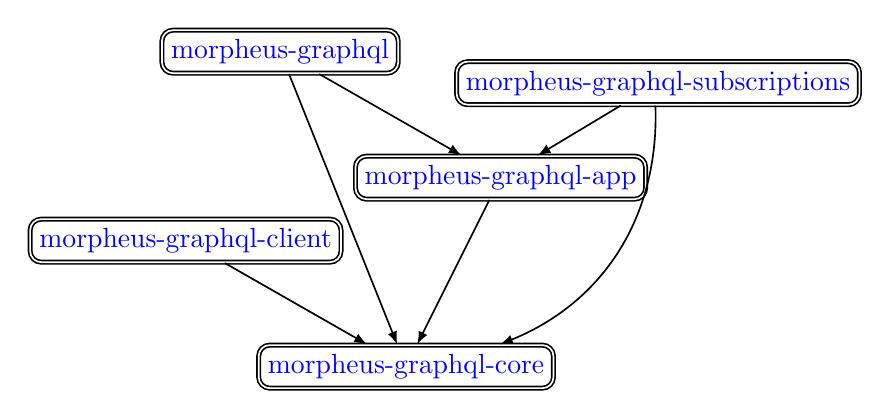
\begin{tikzpicture}[
        scale=.4,
        auto=left,
        -latex ,
        auto ,
        node distance =2 cm and 2cm ,
        % on grid ,
        semithick ,
        package/.style ={ fill=red!20,draw,double,rounded corners ,top color =white ,draw , text=blue , minimum width =1 cm},
    ] 
    \node[package] (core) at (10,0) {morpheus-graphql-core};
    \node[package] (client) at (3,4)  {morpheus-graphql-client};
    \node[package] (app) at (13,6)  {morpheus-graphql-app};
    \node[package] (server) at (6,10)  {morpheus-graphql};
    \node[package] (subs) at (18,9) {morpheus-graphql-subscriptions};
  
    \path (client) edge (core);
    \path (app)  edge (core);
    \path (server)  edge  (core);
    \path (server)  edge  (app);
    \path (subs)  edge  (app);
    \path 
        (subs) 
            edge [bend left =35] 
        (core);  

\end{tikzpicture}
\end{center}
\end{figure}


\section{Derivation}

\input{src/sections/deriving/schema}

%!TEX root = ../../main.tex

\subsection{Mapping Rules}

% \begin{frame}\frametitle{Mapping Rules}

% % The underlying entity of every GraphQL schema is a type. Thereby there are six types of named type definitions and two wrapping types~\cite{gql-spec}. 
% \footnotesize
% \begin{itemize}

%   \li{Positional Constructors} GraphQL fields must always have names~\cite{gql-spec}. 
%   That why we assume that a constructor without field selectors is enumerated like an array.
  
%   \importHS{positional-cons}{Positional Constructors}

%   \li{Unit Type} The unit type indicates the absence of a specific value and serves as a placeholder when no other value exists or is needed~\cite{fsharp-unit}. GraphQL does not provide it~\cite{gql-spec}. 

%   \importGQL{unit-type}{GraphQL Unit Type Definition}

% \end{itemize}
% \end{frame}

\begin{frame}\frametitle{Mapping Wrapping Types}

\begin{itemize}

  \li{Non-Null} GraphQL types are nullable by default: e.g., a scalar string can return either zero or a string value. The non-null type wraps another type and means that the resulting value will never be null~\cite{gql-spec}.


  \li{List} GraphQL List is a collection of homogeneous elements, where the elements are ordered and serialized according to their type~\cite{gql-spec}. 
\end{itemize}

\end{frame}

\begin{frame}\frametitle{Mapping Scalars}

Scalar types represent primitive leaf values in a GraphQL type system. They can be represented as strings. GraphQL offers built-in scalar and enables users to extend the type system with additional scalars with their semantic meaning~\cite{gql-spec}.

Since scalar types have no structural representation, we will impose no restriction and allow any type to represent a scalar type if it has appropriate parse and serialization methods.

\begin{itemize}

  \item Int: Int
  %  This scalar type represents a signed numeric 
    32-bit non-fractional value~\cite{gql-spec}. 

  \item Float: Double
  %  GraphQL-Float represents signed fractions with double precision~\cite{gql-spec}

  \item String: Text
  %  GraphQL String is a regular UTF-8 string for text data~\cite{gql-spec}. Haskell represents strings through the built-in list type. It allows the programmer to use the polymorphic list combinations for complex string manipulations.
  % However, it is also extremely inefficient. An alternative to String is the type Text, which is an array-based string representation that is faster and more compact than String~\cite{string-vs-text,string-types-alexeyshmalko,string-types-fpcomplete,hackage-data-text}. 
  \item Boolean: Bool
  % Since this represents typical Boolean values (true and false)~\cite{gql-spec}, it is represented as a type Bool.
  \item ID:  defined custom data type ID 
  % is a unique identifier that should always be serialized as a String (although it is often numeric)~\cite{gql-spec}. Accordingly, we declare a new data type ID with parse and serialization implementations that meet this specification.
\end{itemize}

\end{frame}

\begin{frame}\frametitle{Mapping Enums}

enum types describe the set of possible independent, unique values~\cite{gql-spec}. They correspond to the algebraic data type with empty fields. The type is only represented as an enum if all its constructors are empty.

\importHS{enum}{GraphQL Enum}
\importGQL{enum}{GraphQL Enum}

\end{frame}

\begin{frame}\frametitle{Mapping Input Object And Field Arguments}

A GraphQL input objects and arguments are is a sets of labeled input values~\cite{gql-spec}. They resemble single constructor Haskell records. 

\importHS{input-object}{GraphQL Input Object in Haskell}
\importGQL{input-object}{Input Object Deity}

\end{frame}
\begin{frame}[allowframebreaks]\frametitle{Mapping Objects}

GraphQL objects are a set of named fields, where fields themselves consist of argument and return type~\cite{gql-spec}. We represent the object types with parameterized records, where the record fields can take function types. This technique allows types to be defined independently of the resolver operations, and the concrete operations can be passed recursively from parent to child. 

\importHS{object-type}{GraphQL Object in Haskell}

\importGQL{object-type}{GraphQL Object in Haskell}

\end{frame}

\begin{frame}[allowframebreaks]\frametitle{Unions}

GraphQL unions represent an object, one of the possible alternative object types, but do not provide guaranteed fields between them~\cite{gql-spec}. 

% While in GraphQL, we only refer to the object type in the list of possible types, in Haskell, we put each of them into a specific constructor. Furthermore, in Haskell, we can create alternative objects only with constructors without defining their types.

\importHS{union}{Union Types}
\begin{itemize}
  \item we unpack constructors, where the name is the concatenation of the type constructor name and the referencing type name. for rest we generate new constructors object.
  \item since GraphQL does not supports empty objects we add every empty object unit field.
\end{itemize}

\importGQL{union}{Union Types}

\end{frame}

% \begin{frame}\frametitle{Determining GraphQL Types in Haskell}
% Compiler applies the following rules with a given execution order to achieve deterministic derivation.
% \begin{enumerate}
%   \li{Scalar, Wrapper, Interface} Derive scalar, wrapper, interface if the type has explicitly specified associated kinds. 
%   \li{Field Arguments} Derive field arguments if the type is used as an argument of the object field. 
%   \li{Enum} Derive enum if all data type constructors are empty.
%   \li{Object} Derive object if the type has a single non-empty constructor, and its parent \footnote{Type A is the parent type of type B if it has a field that refers to type B} is Object or Union. 
%   \li{InputObject} Derive input object if the type has a single non-empty constructor, and its parent is InputObject or Field Arguments.
%   \li{Union} Derive Union if the type has multiple constructors and its parent is Object or Union.
%   \li{Fail} All other types are not supported.
% \end{enumerate}
% \end{frame}

\section{Evaluation}

\begin{frame}[allowframebreaks]\frametitle{Evaluation}


\begin{itemize}
  \li{Maintainability} We use a code-first approach and derive the API from native Haskell types based on data-generic programming. The approach is familiar and reduces boilerplate. The library architecture divides the functionalities into separate, coherent packages. Parameterized resolver types facilitate modular API definitions.
  \li{Reliability} The Haskell compiler primarily achieves type safety. Furthermore we used Template Haskell for schema validity checking. The library meets all the critical parts of the specifications. However, interfaces and directives are still not fully implemented. 

  \li{Efficiency} we used the type \expr{Text} instead of \expr{String}. The library is lazy and only executes the resolvers necessary for the query. 

\end{itemize}
\end{frame}

\begin{frame}\frametitle{Comparison}

Other Haskell libraries provide more extensibility in schema definition than our approach. Besides, the argument chain definitions of the GraphQL API are more flexible than Haskell records for small sets of arguments. However, implementing resolvers for these schemas in our library is simpler because users receive more meaningful error messages, and field values are irrelevant. Besides, our approach is more intuitive and requires less experience than the type-level approach.

There are other libraries in various languages that also have datatype-generic programming to derive GraphQL APIs. However, since we are using Haskell, we have automatically obtained Haskell's lazy and pure nature, which matches the lazy resolvable nature of GraphQL fields. This way, Haskell developers do not need to explicitly consider concurrency and laziness and focus on business logic. 

\end{frame}

\section{Conclusions}

\begin{frame}

\frametitle{Conclusions}

In this work, we presented Morpheus GraphQL, an EDSL for building GraphQL APIs in Haskell. The presented approach provides an easy-to-use interface based on a datatype-generic programming technique and successfully implements the requirements. We chose intuitive design (like Aeson) over extensibility provided by the type-level encoding. 
This gives beginners the ability to quickly learn and implement GraphQL APIs in Haskell while preserving type safety.
The library automatically derives APis from data types, which guarantees type-safe resolver values. We also provide two Template Haskell tools, one of which guarantees schema validity at compile time. The second one imports schemas from GraphQL SDL to facilitate quick start and migration from other languages.
The data resolvers are regular monadic Haskell functions. These resolvers can be extended by arbitrary monads to solve specific problems.  The architecture is divided into small independent packages. Besides, one of the packages, the Morpheus GraphQL client, enables type-safe queries by rejecting invalid queries at compile-time and automatically generating the request and response types.
\end{frame}

\section{Contributions}

\begin{frame}\frametitle{Contributions}

\begin{itemize} 
  
    \li{@Pygmalion} initial name and inspirations

    \li{@krisajenkins} Parser optimization, parameterized resolver types
    
    \li{@theobat} custom wrapping types and the library Massalia

\end{itemize}

\end{frame}
%!TEX root = ../main.tex
\section{Example}

\begin{frame}\frametitle{Morpheus}

repository: \url{https://github.com/nalchevanidze/morpheus-haxl-example}

\end{frame}
\setLayout{blank}
%!TEX root = ../../main.tex

\section*{Thanks}

\begin{frame}
    
    \centering
    \vspace{5pt}
    
    \textbf{\Huge Danke!}
 
    \ \\
    \ \\
    \textbf{Fragen oder Anregungen?}
    
    \text{\footnotesize d.nalchevanidze@gmail.com}
    
    \vspace{5pt}
    \begin{figure}
      \centering\includegraphics[height=30pt]{assets/logo/uhh.pdf}
    \end{figure}
\end{frame}
\setLayout{titlepage}
\titlepage
\setLayout{regular} 

\begin{frame}[plain, noframenumbering,allowframebreaks]{References}
    \printbibliography
\end{frame}

\end{document}